\def\year{2020}\relax

\newcommand{\tuple}[1]{\ensuremath{\left \langle #1 \right \rangle }}


% These are the instructions for authors for IJCAI-19.

\newcommand{\qed}{\hfill\ensuremath{\blacksquare}}
\newcommand{\astar}{A$^*$}
\newcommand{\epea}{EPEA$^*$}
\newcommand{\SAS}{SAS$^+$}
\newcommand{\wastar}{WA$^*$}
\newcommand{\arastar}{ARA$^*$}
\newcommand{\open}{\textsc{Open}}
\newcommand{\closed}{\textsc{Closed}}
\newcommand{\eff}{\textit{eff}}
\newcommand{\pre}{\textit{pre}}
\newcommand{\solvable}{\textit{S}}
\newcommand{\plannable}{\textit{P}}
\newcommand{\true}{\textit{T}}
\newcommand{\false}{\textit{$\bot$}}
\newcommand{\AS}{AS\xspace}


%File: formatting-instruction.tex

\documentclass[letterpaper]{article} % DO NOT CHANGE THIS
\usepackage{aaai20}  % DO NOT CHANGE THIS
\usepackage{times}  % DO NOT CHANGE THIS
\usepackage{helvet} % DO NOT CHANGE THIS
\usepackage{courier}  % DO NOT CHANGE THIS
\usepackage[hyphens]{url}  % DO NOT CHANGE THIS
\usepackage{graphicx} % DO NOT CHANGE THIS
\urlstyle{rm} % DO NOT CHANGE THIS
\def\UrlFont{\rm}  % DO NOT CHANGE THIS
\usepackage{graphicx}  % DO NOT CHANGE THIS
\frenchspacing  % DO NOT CHANGE THIS
\setlength{\pdfpagewidth}{8.5in}  % DO NOT CHANGE THIS
\setlength{\pdfpageheight}{11in}  % DO NOT CHANGE THIS

\usepackage{subcaption} 
\usepackage{tabularx}
\usepackage{array}

\usepackage{booktabs}% for \toprule, \midrule, \bottomrule, and \cmidrule macros
\usepackage{amsmath} % for \text macro

%\usepackage[pdfencoding=auto]{hyperref}
\usepackage[draft]{hyperref}


\usepackage{amsmath}
\usepackage{booktabs}

\urlstyle{same}

\usepackage{algorithmic}
\usepackage{booktabs}
\usepackage[usenames,dvipsnames]{xcolor}
\usepackage[ruled,vlined,linesnumbered]{algorithm2e}
\usepackage{amsmath}
\usepackage{amsthm}
\usepackage{url}
\usepackage{multirow}
\usepackage[super]{nth}

\usepackage{xspace}


%
% Add comments in the text
%
\newboolean{showcomments}
%\setboolean{showcomments}{true}
\setboolean{showcomments}{false}

\ifthenelse{\boolean{showcomments}}
  {\newcommand{\nb}[3]{
  {\color{#2}\small\fbox{\bfseries\sffamily\scriptsize#1}}
  {\color{#2}\sffamily\small$\triangleright~$\textit{\small #3}$~\triangleleft$}
  }
  }
  {\newcommand{\nb}[3]{}
  }

\newcommand\Roni[1]{\nb{\textbf{Roni:}}{red}{#1}}
\newcommand\Omri[1]{\nb{\textbf{Omri:}}{orange}{#1}}


\newcommand{\inlinecite}[1]{\citeauthor{#1} \shortcite{#1}}

% \nocopyright
%PDF Info Is REQUIRED.
% For /Author, add all authors within the parentheses, separated by commas. No accents or commands.
% For /Title, add Title in Mixed Case. No accents or commands. Retain the parentheses.
 \pdfinfo{
/Title (Algorithm Selection for Optimal Classical MAPF)
/Author (Submission XXX)
} %Leave this	
% /Title ()
% Put your actual complete title (no codes, scripts, shortcuts, or LaTeX commands) within the parentheses in mixed case
% Leave the space between \Title and the beginning parenthesis alone
% /Author ()
% Put your actual complete list of authors (no codes, scripts, shortcuts, or LaTeX commands) within the parentheses in mixed case. 
% Each author should be only by a comma. If the name contains accents, remove them. If there are any LaTeX commands, 
% remove them. 

% DISALLOWED PACKAGES
% \usepackage{authblk} -- This package is specifically forbidden
% \usepackage{balance} -- This package is specifically forbidden
% \usepackage{caption} -- This package is specifically forbidden
% \usepackage{color (if used in text)
% \usepackage{CJK} -- This package is specifically forbidden
% \usepackage{float} -- This package is specifically forbidden
% \usepackage{flushend} -- This package is specifically forbidden
% \usepackage{fontenc} -- This package is specifically forbidden
% \usepackage{fullpage} -- This package is specifically forbidden
% \usepackage{geometry} -- This package is specifically forbidden
% \usepackage{grffile} -- This package is specifically forbidden
% \usepackage{hyperref} -- This package is specifically forbidden
% \usepackage{navigator} -- This package is specifically forbidden
% (or any other package that embeds links such as navigator or hyperref)
% \indentfirst} -- This package is specifically forbidden
% \layout} -- This package is specifically forbidden
% \multicol} -- This package is specifically forbidden
% \nameref} -- This package is specifically forbidden
% \natbib} -- This package is specifically forbidden -- use the following workaround:
% \usepackage{savetrees} -- This package is specifically forbidden
% \usepackage{setspace} -- This package is specifically forbidden
% \usepackage{stfloats} -- This package is specifically forbidden
% \usepackage{tabu} -- This package is specifically forbidden
% \usepackage{titlesec} -- This package is specifically forbidden
% \usepackage{tocbibind} -- This package is specifically forbidden
% \usepackage{ulem} -- This package is specifically forbidden
% \usepackage{wrapfig} -- This package is specifically forbidden
% DISALLOWED COMMANDS
% \nocopyright -- Your paper will not be published if you use this command
% \addtolength -- This command may not be used
% \balance -- This command may not be used
% \baselinestretch -- Your paper will not be published if you use this command
% \clearpage -- No page breaks of any kind may be used for the final version of your paper
% \columnsep -- This command may not be used
% \newpage -- No page breaks of any kind may be used for the final version of your paper
% \pagebreak -- No page breaks of any kind may be used for the final version of your paperr
% \pagestyle -- This command may not be used
% \tiny -- This is not an acceptable font size.
% \vspace{- -- No negative value may be used in proximity of a caption, figure, table, section, subsection, subsubsection, or reference
% \vskip{- -- No negative value may be used to alter spacing above or below a caption, figure, table, section, subsection, subsubsection, or reference


\usepackage{xspace}
\usepackage{acronym}

\usepackage{graphicx}
\graphicspath{ {images/} }

\setcounter{secnumdepth}{2} %May be changed to 1 or 2 if section numbers are desired.

% The file aaai20.sty is the style file for AAAI Press 
% proceedings, working notes, and technical reports.
%
\setlength\titlebox{2.5in} % If your paper contains an overfull \vbox too high warning at the beginning of the document, use this
% command to correct it. You may not alter the value below 2.5 in
%\title{Probabilistic Robust Multi-Agent Path Finding}
%Your title must be in mixed case, not sentence case. 
% That means all verbs (including short verbs like be, is, using,and go), 
% nouns, adverbs, adjectives should be capitalized, including both words in hyphenated terms, while
% articles, conjunctions, and prepositions are lower case unless they
% directly follow a colon or long dash

\newcommand{\OPEN} {{\textsc{Open}}}

\newtheorem{definition}{Definition}
\newtheorem{lemma}{Lemma}
\newtheorem{theorem}{Theorem}
\newcommand{\ignore}[1]{}

\author{Submission \#90}


%Written by AAAI Press Staff\textsuperscript{\rm 1}\thanks{Primarily Mike Hamilton of the Live Oak Press, LLC, with help from the AAAI Publications Committee}\\ \Large \textbf{AAAI Style Contributions by
%Pater Patel Schneider,} \\ \Large \textbf{Sunil Issar, J. Scott Penberthy, George Ferguson, Hans Guesgen}\\ % All authors must be in the same font size and format. Use \Large and \textbf to achieve this result when breaking a line
%\textsuperscript{\rm 1}Association for the Advancement of Artificial Intelligence\\ %If you have multiple authors and multiple affiliations
% use superscripts in text and roman font to identify them. For example, Sunil Issar,\textsuperscript{\rm 2} J. Scott Penberthy\textsuperscript{\rm 3} George Ferguson,\textsuperscript{\rm 4} Hans Guesgen\textsuperscript{\rm 5}. Note that the comma should be placed BEFORE the superscript for optimum readability
%2275 East Bayshore Road, Suite 160\\
%Palo Alto, California 94303\\
%publications20@aaai.org % email address must be in roman text type, not monospace or sans serif

\begin{document}




%%
%% The "title" command has an optional parameter,
%% allowing the author to define a "short title" to be used in page headers.
\title{Algorithm Selection for Optimal Multi-Agent Pathfinding}


%\author{}


%%
%% The "author" command and its associated commands are used to define
%% the authors and their affiliations.
%% Of note is the shared affiliation of the first two authors, and the
%% "authornote" and "authornotemark" commands
%% used to denote shared contribution to the research.

% \authornote{Both authors contributed equally to this research.}
% \email{trovato@corporation.com}
% \orcid{1234-5678-9012}
% \author{G.K.M. Tobin}
% \authornotemark[1]
% \email{webmaster@marysville-ohio.com}
% \affiliation{%
%   \institution{Institute for Clarity in Documentation}
%   \streetaddress{P.O. Box 1212}
%   \city{Dublin}
%   \state{Ohio}
%   \postcode{43017-6221}
% }

% \author{
% Eran Hershkovich,\textsuperscript{\rm 1}
% Roni Stern,\textsuperscript{\rm 1}
% Rui Abreu,\textsuperscript{\rm 1}
% Amir Elmishali,\textsuperscript{\rm 2}
% \textsuperscript{\rm 1}Ben Gurion University of the Negev,
% \textsuperscript{\rm 2}University of Lisbon\\
% eranhe@post.bgu.ac.il
% sternron@post.bgu.ac.il,
% rui@computer.org,
% amir9979@gmail.com,
% }

%\Eran{hope this is the right format}
\author{Submission \#90}

\maketitle

%%
%% The abstract is a short summary of the work to be presented in the
%% article.
\begin{abstract}
%Research on multi-agent path finding (MAPF) has been flourishing, with new algorithms or algorithmic improvements appearing every year. Specifically, 
The challenge of finding an optimal solution to a multi-agent path finding (MAPF) problem has attracted significant academic and industrial interest in recent years. While the problem is NP-Hard, modern optimal MAPF algorithms can scale to solve problems with hundreds of agents. 
Nevertheless, no single optimal MAPF algorithm dominates all benchmarks problems, and there are no clear, provable, guidelines for when each algorithm should be used. 
To address this, %we apply a data-driven approach and 
present the first successful Algorithm Selection (\AS) model for optimal MAPF. 
We propose two approaches for learning a AS model. The first approach uses a standard supervised learning algorithm 
with a set of handcrafted MAPF-specific features. The second approach, casts a MAPF problem to an image and applies a deep Convolutional Neural Network to classify it. 
We evaluate both approaches over a large dataset and show that using an \AS model to select which algorithm to use for each instance results in solving more problems and in a shorter runtime compared to the state of the art. 
%The and machine learning techniques in order to automatically select the most suited solver for a given MAPF problem. We demonstrate the effectiveness of our method at being able to outperform any individual MAPF algorithm on MAPF benchmarks.
\end{abstract}

%%
%% This command processes the author and affiliation and title
%% information and builds the first part of the formatted document.

\section{Introduction}

% What is MAPF
A \emph{classical multi-agent pathfinding (MAPF)} problem with $k$ agent~\cite{stern2019multiagent} is defined by a tuple $\langle G,s,t \rangle$, where $G = (V,E)$ is an undirected graph, 
$s: [1,\ldots,k] \rightarrow V$ maps an agent to its source vertex, 
and $t: [1,\ldots,k] \rightarrow V$ maps an agent to its target vertex. 
Each agent starts in its source vertex. In every time, an agent either \emph{waits} in its current vertex or \emph{moves} to one of the vertices adjacent to it. 
A solution to a classical MAPF problem is a sequence of wait/move actions for each agent such that the agents reach their targets without colliding with each other. 
In this work, we focus on the problem of finding an \emph{optimal} solution to a given MAPF problem. 
This problem is known to be NP Hard for various common optimization criteria~\cite{DBLP:conf/aaai/Surynek10,DBLP:conf/aaai/YuL13}. Nevertheless, Classical MAPF and its many extensions have important applications in robotics, autonomous vehicles, and automated warehouses, 
and hence, many optimal MAPF algorithms have been proposed~\cite{felner2017search,ma2017buzz}. 
Nevertheless, no algorithm has emerged to dominate all others. 
In fact, very little is known for how to choose which optimal MAPF algorithm to use for a given classical MAPF problem. 

% No universal winner. Our contribution: the first algorithm selection algorithm for search-based optimal MAPF. 

To close this gap, we propose a data-driven approach to learn an \emph{Algorithm Selection} (AS) model for optimal MAPF. 
An AS model accepts a portfolio of optimal MAPF algorithms $\mathcal{A}$ and 
a MAPF problem $\Pi$, and outputs an algorithm in $\mathcal{A}$ for solving $\Pi$. Our main objective is to create an \AS model that chooses an algorithm that solves $\Pi$ in minimal runtime. 
We explore two approaches for creating such a model. 
In the first approach, we use XGBoost~\shortcite{chen2016xgboost}, a state of the art tree-based supervised learning algorithm, with a set of handcrafted MAPF-specific features. In the second approach, we follow the work of Sigurdson et al.~\cite{sigurdson2019deep} and cast the given MAPF problem to an image, and then train a deep Convolution Neural Networks (CNN) to select the appropriate optimal MAPF algorithm. We evaluate the AS models created by both approaches over a dataset with 39,000 samples across 28 grid types. 
The results show that the best AS model selects the best algorithm in over 65\% of the cases, and using the selected MAPF algorithm significantly outperforms all the state of the art optimal MAPF algorithms in our portfolio. For example, using the best AS model we were able to solve 93\% of all problems in our benchmark under 5 minutes, while the best MAPF algorithm solved only 82\%. 


It is worth noting that our portfolio only contains search-based MAPF algorithms. That is, we do not consider MAPF algorithms that are based on compilation to Boolean Satisfiability~\cite{surynek2016efficient,DBLP:conf/socs/BartakS19}, constraints programming~\cite{DBLP:conf/ictai/BartakZSBS17}, and SMT~\cite{surynek2019unifying,erdem2013general}. Such algorithms are known to be highly effective in some domains, while less so in others. Nevertheless, using our best AS model can be viewed as the first universal winner among all search-based solver, and the proposed approach can be easily applied to include other MAPF algorithms in the portfolio. 

%Our portfolio only contains search-based MAPF algorithms, namely ICTS~\cite{sharon2013increasing} and several variants of \astar~\cite{hart1968formal} and CBS~\cite{sharon2015conflict}. That is, we do not consider MAPF algorithms that are based on compilation to Boolean Satisfiability~\cite{surynek2016efficient,DBLP:conf/socs/BartakS19}, constraints programming~\cite{DBLP:conf/ictai/BartakZSBS17}, and SMT~\cite{surynek2019unifying,erdem2013general}. Such algorithms are known to be highly effective in some domains, while less so in others. Nevertheless, our algorithm can be viewed as the first universal winner among all search-based solver, and the proposed approach can be easily applied to include other MAPF algorithms in the portfolio. 


% Prior work: algorithm selection for suboptimal MAPF
To the best of our knowledge, the only prior work on AS for MAPF is by Sigurdson et al.~\shortcite{sigurdson2019deep}. They focused on finding any solution to a given MAPF problem while we aim to find optimal solutions, and thus our portfolio consists only optimal MAPF algorithm. Also, we explore a range of approaches to learn an AS model. 






\section{Background}

In this work, we consider classical MAPF problems in a graph that represents a 4-neighborhood grid~\cite{stern2019multiagent}. 
Time is discretized and each action -- wait or move -- takes one time step. 
A collision between single-agent plans occurs if there is either a vertex, edge, and swapping conflicts between them, i.e., the agents cannot occupy the same vertex, the same edge, or swap locations, at the same time, respectively. 
When an agent reaches its target, it stays there and blocks other agents from passing through that vertex.\footnote{However, an agent can reach its target and then move away from it to allow another agent to pass. Afterward, the agent must return to its target since eventually all agents must end up in their targets.} 
The \emph{cost} of a solution to a MAPF problem is the number of move/wait actions all agents perform until all agents reach their target. This is known as the \emph{sum-of-costs} objective. 
An optimal MAPF algorithm is an algorithm that is guaranteed to return a lowest-cost solution.  


%sum of actions itto a 
% Problem Definition
%Let $\mathcal{A}$ be a portfolio of optimal MAPF algorithms. For a MAPF problem $\pi$ and MAPF algorithm $A\in\mathcal{A}$, let Time($\pi,A$) be the runtime it takes for $A$ to solve $\pi$. The problem we address in this work is as follows: for a given MAPF problem $\pi$ we wish to return the algorithm $A$ that minimizes Time($\pi, A$). 


\subsection{Algorithms in the Portfolio}
In this work, we used the following diverse set of optimal search-based MAPF algorithms: 
(1) \astar~\cite{hart1968formal} with the Operator Decomposition (OD) and Independence Detection (ID) MAPF-specific enhancements~\cite{standley2010finding}, 
(2) Enhanced Partial Expansion \astar (\epea), which is an \astar variant designed for state spaces with a large branching factor that was shown to be effective for MAPF~\cite{goldenberg2014enhanced}, 
(3) Increasing Cost Tree Search (ICTS)~\cite{sharon2013increasing}, 
(4) Conflict-Based Search (CBS)~\cite{sharon2015conflict}, (5) MA-CBS, which improves CBS by merging agents to a meta-agent when needed, 
and (6) a state-of-the-art variant of CBS that includes a recently proposed heuristic~\cite{li2019improved} and conflict bypassing and prioritization~\cite{boyarski2015icbs}. 
The latter will be referred to in this paper as CBS-H. 
For an overview of search-based optimal MAPF algorithms including these algorithms see Felner et al.~\cite{felner2017search}. 



\subsection{Algorithm Selection (AS)}
% Some background on Algorithm Selection 

Algorithm Selection (\AS) is the problem of selecting the best algorithm from a given set of algorithms on a per-instance basis~\cite{rice1976algorithm}. 
\AS has been successfully solved for a range of optimization and satisfaction problems~\cite{kotthoff2016algorithm,kerschke2019automated}. A notable example is SATZilla~\cite{xu2012satzilla2012}, which is a highly successful algorithm for generating an AS model for solving Boolean Satisfiability problems. 
% Algorithm selection as oppose to algorithm configuration
%Note that \AS is different from Automatic Algorithm Configuration (AAC)~\cite{hutter2009paramils}. In AAC, the challenge is to automatically generate an optimized algorithm given a set of possible configurations for that algorithm. By contrast, in \AS, one has a set of algorithms but cannot mix their components. Nevertheless, some of the techniques in AAC can be used for Algorithm Selection and vice versa. 

% Approaches: regression or classification 
Supervised machine learning is the current standard method for generating effective \AS models. 
Such learning-based methods can be split into two major approaches. 
The first approach is based on \emph{effort estimation}. That is, the data in the training set is used to learn a regression model for each algorithm $A\in\mathcal{A}$ that aims to predict the runtime it will take $A$ to solve a given problem. 
The corresponding \AS model chooses the algorithm predicted to require the least amount of runtime to solve the given problem.  
%Algorithms that follow this approach are fundamentally solving an \emph{effort estimation} problem. 
%The common approach to solve this problem is by considering data from past executions and applying a \emph{regression} algorithm, e.g., one that trains a neural network or fits a polynomial regression function. 
A different approach to learn an \AS model is to directly train a multi-class classifier to predict who is the best algorithm for a given problem.  %Off-the-shelf classification algorithms for this include tree-based algorithms such as Random Forest~\cite{liaw2002classification}, XGBoost~\cite{chen2016xgboost}, and neural networks.\footnote{Note that Random Forest and XGBoost also have versions that solve regression problems.}. 
To differentiate between these two approaches, we refer to the former as the \emph{regression approach} and the latter as the \emph{classification approach}. 


Both approaches are known to have limitations. 
The regression approach is inherently more difficult, since the space of mistakes is larger (all possible runtimes), and predicting runtimes is considered a noisy target for regression models. The classification approach outputs a single algorithm for a given MAPF problem, so it cannot be sensitive to cases where two algorithms perform similarly. %Moreover, incorrect selections can have different effects on overall performance. 
There are more sophisticated approaches that aim to mitigate these limitations. For example, Xu et al.~\shortcite{xu2012satzilla2012} proposed to mitigate the limitation of the classification approach by learning a cost-sensitive binary classification model for every pair of  solvers~\cite{xu2012satzilla2012}. To select an algorithm for a given problem $\Pi$, the solvers are ranked according to the number of times each of them has been chosen by the classifiers for $\Pi$, and the highest-ranking solver is returned. 
We experimented with this approach in our domain and did not observe any improvement. Since this approach is also significantly more costly in terms of training time, we focus in the rest of this paper on the more fundamental regression and classification approaches.  

%\emph{Ordinal regression methods}~\cite{gutierrez2015ordinal}, aim to bypass these challenges by learning an AS model that is able to predict the order of algorithms in respect to their running times on a given problem. Yet, it is well-known that prior knowledge about the pair-wise class distances (i.e., the distance between fastest and second-fastest algorithm) has significant effects on performance, as shown by \cite{sanchez2013exploitation}. Thus, in this paper we explore only the classification and regression approaches.




%At the field of meta-learning, algorithm selection methods (CITE) attempts to identify the most suitable classifier (and parameter settings) for a given classification problem. Recent advances at this field explores the balancing between accuracy of the selected classifier and the training time it took to train it (\cite{brazdil2003ranking}, \cite{}, cite{}). Inspired by their methods, at this paper we detail our methods to balance between accuracy and running time at the field of MAPF algorithm selection.\
%\subsubsection{Multi Task Training} Train one model with two tasks - predict the runtime for each algorithm + classify the best algorithm. Specify about loss weights. Give in short details about training the CNN while trying to predict the extracted features.
% \subsubsection{Relative Runtime As Probability} TODO: explain on a method: Normalize the outputs to be probability distribution for each example and use classification with log softmax output and cross enropy loss. For example - If for a given instance the results of algorithms was: 1. 10 mili, 2. 11 mili, 3. 100 mili, 4. 1000 mili, 5. 180000 mili, then the target for the classification problem will be the normalized probability (1 - relative part of time to sum of al time), and using the log softmax activation (log in order to not be biased towards the max) to predict this probability distribution. Thus effectively the balancing between accuracy (fastest solver thus highest probability) and coverage (never pick low probability because high loss) is achieved.  Why this balancing not achieved using regression? Because regression have multiple problems (censored data, "noisiness" regarding to scale of miliseconds..)\Roni{Do we have experiments for this?}\subsubsection{Experiment with SATZilla2012 cost-sensitive learning approach} \cite{xu2012satzilla2012} used cost-sensitive binary classification model for every pair of solvers. Then, at prediction, they used those classifiers as selecting the solver with the highest number of votes (i.e., highest number of times being predicted). We experimented with this approach and did not seen improvement. Thus, due to the large time it takes to train all pairs and the fact that it didn't gave us better results, we don't use this method.



\begin{figure*}[t]
\minipage{0.2\textwidth}
    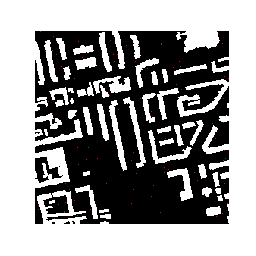
\includegraphics[width=\linewidth]{images/Berlin_1_256-71-5-label1.png}  
    %\caption{A really Awesome Image}\label{fig:awesome_image1}
    \caption{MAPF problem represented as an image.}% Red and green pixels are source and target vertices of the agents.}
    \label{fig:cnn-image}
\endminipage\hfill
\minipage{0.25\textwidth}
\resizebox{\textwidth}{!}{
\begin{tabular}{@{}lrrr@{}}
\toprule
Model                    & Accuracy & Coverage & Total RT \\ \midrule
 \astar+OD+ID & 0.00 & 0.73 & 12,459 \\
 EPE\astar & 0.12 & 0.79 & 9,871 \\ 
 ICTS & 0.10	& 0.78 & 10,570 \\
 CBS & 0.00 & 0.59 & 17,447 \\
 MA-CBS & 0.26 & 0.53	& 19,952 \\
 CBS-H & 0.50 & 0.83 & 8,016 \\ 
 \midrule
 Random & 0.16 & 0.71 & 13,215 \\  
 CNN Rg. & 0.51 & 0.88 & 6,210 \\ 
 XGBoost Rg. & 0.51	& 0.82 & 8,410 \\
 CNN Cl. & 0.55 & 0.91 & 5,122 \\
 XGBoost Cl. & 0.66 & 0.93 & 4,307 \\
 \midrule
 Oracle & 1.00 & 100.00 & 1,649 \\
\bottomrule
\end{tabular}
}
  \caption{Results for all models across all the test set.}
  \label{table:allResults}  
\endminipage\hfill
\minipage{0.45\textwidth}%
    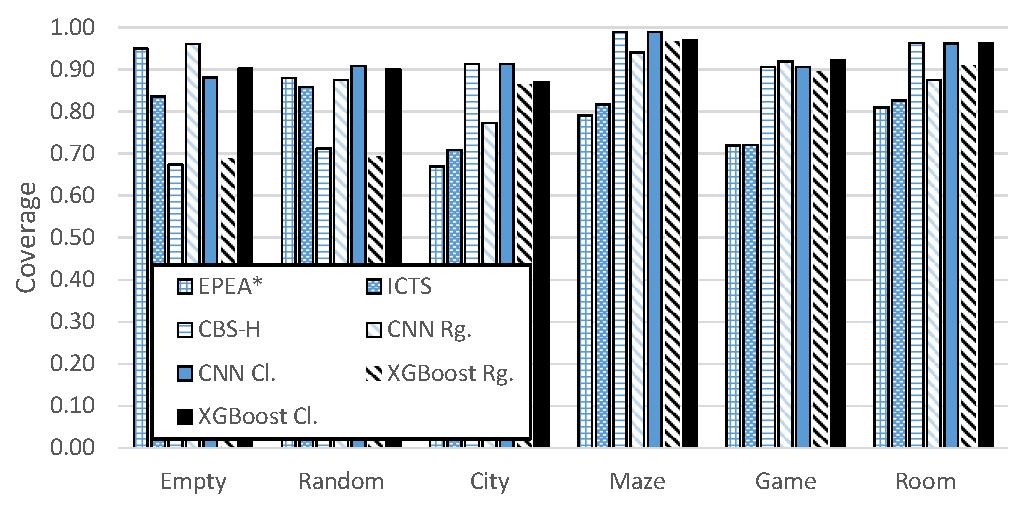
\includegraphics[width=\columnwidth]{coverageByMap.pdf}
    \caption{Coverage results, split by grid types.}
    \label{fig:coverageByMap}  
\endminipage
\end{figure*}
%\Roni{TODO: Explain algorithms}

\section{Learning \AS Models for Optimal MAPF}
The first learning approach we explore uses a state-of-the-art tree-based learning algorithm, namely XGBoost~\cite{chen2016xgboost}, with a set of handcrafted features specifically designed for MAPF. 
% Describe the features
A key factor in the effectiveness of XGBoost, and in general supervised learning algorithms, is the set of features extracted from every instance. We created the following sets of MAPF-specific features. 

\subsection{Handcrafted MAPF Features}
\label{sec:xgbsoot}
The first set of features describes the grid. This set of features include the following features:
(1) the number of rows and columns in the grid (denoted GridRows and GridColumns), 
(2) the number of blocked cell in the grid (NumOfObstacles), 
and (3) the ratio of blocked cells, i.e., $\frac{NumOfObstacles}{GridRows\cdot GridCols}$. The last feature is called ObstacleDensity. 
The next set of features is derived from the number of agents and its relation to the grid size. This set of features include 
(1) the number of agents ($k$), denoted NumOfAgents, 
(2) the branching factor of a naive \astar search, i.e., $5^k$, 
and (3) the number of agents divided by the number of empty cells in the grid, i.e. cells without an obstacle. I.e., $\frac{k}{|V|}$.\footnote{Note that $V$ is the set of vertices in the graph, which is the number of cells that are not blocked by an obstacle.} The last two features are called BranchingFactor and AgentSparsity. 
The last set of features we used attempts to capture the shortest distances between the agents' source and target vertices. 
Let $\delta(v,v')$ be the length of the shortest path in the grid from $v$ to $v'$. 
The average, maximal, and minimal distance in the grid from source to target over of all agents, i.e.,
$\sum_{i=1}^k\delta\big(s(i),t(i)\big)/k$, 
$\max_{i=1}^k\delta\big(s(i),t(i)\big)$, and 
$\min_{i=1}^k\delta\big(s(i),t(i)\big)$, respectively, are part of this final set of features. 
We call these three features AvgDistanceToGoal, MaxDistanceToGoal, and MinDistanceToGoal, respectively. 
Also in this set of features are the average distance between the source vertices of all agents, i.e., 
    \begin{equation}
            \sum_{i=1}^{k-1}\sum_{j=i+1}^k 2\delta\big(s(i),s(j)\big)/\big(k\cdot (k-1)\big)
    \end{equation}
This feature is called AvgStartDistances. The AvgGoalDistances feature is defined similarly with respect to the average distance between the agents' target vertices. 
The last feature in this set of features is the ratio of open grid cells that are on a shortest path from the source to the target of at least one of the agents. We call this feature CellsAtSPRatio. 
%The first three features in this set are aimed to characterize MAPF problems in which the solution will contain longer of shorter sequences of actions. 
%The last three features in this set are aimed to characterize MAPF problems in which the agents are expected to conflict in specific cells. 

We used the above sets of features and created two \AS models with XGBoost~\cite{chen2016xgboost}, one following the classification approach for \AS and the other following the regression approach. We call the resulting \AS models 
\emph{XGBoost Classification} (XGBoost Cl.) and
\emph{XGBoost Regression} (XGBoost Rg.), respectively. 

%Following the classification approach for \AS, we used XGBoost to train a classification model using all these sets of features, where the label of every MAPF problem is the algorithm that solved it fastest.We call the resulting \AS model \emph{XGBoost Classification} (XGBoost Cl.). In addition, we used the same learning algorithm and features to create an alternative \AS model that follows the regression approach for \AS. In this case, we created a regression model for every algorithm in our portfolio, where the label it aimed to predict is the algorithm's runtime. Then, to choose which algorithm to select we run all these regression models and returned the one that predicted the minimum runtime. We call the resulting \AS model \emph{XGBoost Regression} (XGBoost Rg.). 
%\Roni{Maybe remove the above as it was said, to some extent}



\subsection{Deep Learning MAPF Images}


The second learning approach we explore 
maps a given MAPF problem to an image and then use a Convolutional Neural Network (CNN) to classify it. 
Specifically, we follow Sigurdon et al.'s~\cite{sigurdson2019deep} recent work on \AS for non-optimal MAPF, and use an image to represent a MAPF problem, as follows. 
Blocked and unblocked cells are represented by white and black pixels, respectively. 
Source and target vertices are represented by green and red pixels, respectively.
We resize the resulting image such that it fits into the network input layer, which in our case was set to 224x224x3.\footnote{The last dimension indicates the color of the pixel} An example of such an image is Figure~\ref{fig:cnn-image}. 



There are many CNN architectures for image classification. 
We used the VGG-16 architecture~\cite{simonyan2014very}, which is a modern CNN architecture that is commonly used in the image recognition literature.  %Figure~\ref{fig:vgg} illustrates this architecture. 
In addition, to improve runtime and model accuracy, we made the following adjustments to this architecture. 
First, we added a global average pooling (GAP) layer~\cite{lin2013network} after the last convolution layer. 
After the GAP layer, we added a fully connected layer with 64 neurons to gradually reduce dimensionality towards the output layer, which contained 6 neurons, one per algorithm in our portfolio. 



Using the MAPF image and the CNN architecture described above, we created two \AS models: one following the classification approach and the other following the regression approach. We call the resulting \AS models \emph{CNN Classification} (CNN Cl.)
and \emph{CNN Regression} (CNN Rg.). We note that for CNN Rg., we trained a single CNN so that it accepts a MAPF problem and every output neuron is associated with one of the MAPF algorithms in our portfolio and should output the runtime for the corresponding algorithm on the given MAPF problem. To do so, we use the multi-output regression learning~\cite{borchani2015survey}, which is known to work well with neural networks. 
%The trained CNN was used to select an algorithm from our portfolio by choosing the MAPF algorithm predicted to have the lowest runtime. We call the resulting \AS model \emph{CNN Regression} (CNN Rg.).

%For the classification approach, we used a one-hot encoding of the output layer, labellling the training set as explained for XBoost Cl. We call the resulting \AS model \emph{CNN Classifiaction} (CNN Cl.). 
%For the regression approach, we trained a single CNN so that it accepts a MAPF problem and every output neuron is associated with one of the MAPF algorithms in our portfolio and should output the runtime for the corresponding algorithm on the given MAPF problem. To do so, we use the multi-output regression learning~\cite{borchani2015survey}, which is known to work well with neural networks. The trained CNN was used to select an algorithm from our portfolio by choosing the MAPF algorithm predicted to have the lowest runtime. We call the resulting \AS model \emph{CNN Regression} (CNN Rg.).

\subsection{Dataset}
% Training set source
%\Roni{Where the data came from}
To train and evaluate the \AS models we proposed, we used the publicly available grid-based MAPF benchmark, detailed in~\cite{stern2019multiagent}. 
This benchmark contains 28 grids including 10 grids from popular video games, 3 city maps (Berlin, Boston, Paris), 4 maze-like grids, 3 grids that arranged as rooms with narrow doors between them, 4 open grids, and 4 open grids with randomly placed obstacles. 


This benchmark also includes a set of 25 \emph{scenario} files for each grid. A scenario file contains source and target locations for up to 1,000 agents (where possible). 
We use this scenario file as suggested by Stern et al.~\cite{stern2019multiagent}, that is, we use each algorithm to solve MAPF problems on the chosen grid with one agent, two agents, and so on until the runtime required to solve the problem reaches a timeout of 5 minutes. 
Problems that no algorithm in our portfolio could solve under this time limit were discarded. 
We recorded the runtime of every algorithm in every run, and whether the algorithm has reached a timeout or not.
The resulting dataset consists over 39,000 instances.
Importantly, since scenarios are solved incrementally, a simple random split of the dataset to train and test introduced unfair bias in favor of our \AS algorithms. Thus, we used 30\% of the scenarios as the held-out test set, which verifies that data from the same scenario is not used in both training and testing. 

Our dataset poses a challenge to the regression approach for \AS: how to consider the runtime of an algorithm that failed to solve a problem? This type of data is called \emph{censored data}, and methods to deal with it has been studied, e.g., for survival analysis. Standard methods include removing the censored data, treating it as uncensored (i.e., setting the timeout time as the runtime), as well as sophisticated iterative method~\cite{schmee1979simple}). Treating such data as uncensored worked best for us. %our dataset.








\section{Experimental Results}
% Overall results

We used the following metrics to evaluate the proposed \AS models: accuracy, coverage, and total runtime. 
\emph{Accuracy} is the ratio of problems that the \AS model correctly selected the fastest algorithm in the portfolio for this problem. 
\emph{Coverage} is the ratio of problems solved within the 5 minute timeout using the algorithm selected by the evaluated model. 
\emph{Total runtime} (Total RT) is the overall runtime, in minutes, it took to solve all problems in our test set, choosing for every problem the algorithm selected for it by the evaluated model. 
% Note that this metric is cannot replace the coverage metric, since the runtime is always capped at 5 minutes, even if the problem was not solver. Yet, it gives a quantitative measurement of the time the \AS  algorithm would save on a dataset with a certain captime value. 




\subsection{Accuracy, Coverage, and Total RT Results}
Table~\ref{table:allResults} shows the accuracy, coverage, and total RT for all evaluated algorithms across all scenarios in our test set. For reference, the upper portion of the table shows the results of choosing the same algorithm for all problems. 
Thus, accuracy in this context is the ratio of problems in which that algorithm solved first. \emph{Oracle} and \emph{Random} are also given for comparison purposes: Oracle always chooses the correct MAPF algorithm and Random chooses one randomly. The accuracy of Oracle is 1 and that of Random is one over the number of algorithms in our portfolio. 


% Analyze the results.
The results in Table~\ref{table:allResults} show 
that most \AS models yield better results than every individual algorithm in our portfolio across all parameters. For example, the coverage and total RT of CBS-H is 0.83 and 8,016, respectively, while both CNN classification and XGBoost classification had a coverage higher than 0.9 and a total RT lower than 5,122. 


Comparing the different \AS models, we see that the classification approach yielded better results compared to the regression approach. For example, the coverage of XGBoost regression is 0.82 while it is 0.93 for XGBoost classification. 
% This observation is supported by research on \AS in other fields, where directly learning a classifier is better than indirectly learning one via effort estimation. 
% \Roni{Find a ref?}
Comparing XGBoost and CNN classification models 
show that while XGBoost is significantly more accurate, it only has a modest advantage in terms of coverage and total RT. 



%To gain a deeper insight into the performance of the different models, 
Figure~\ref{fig:coverageByMap} shows coverage ($y$-axis) of the best models from each family of algorithms for different grid types. 
The results highlight the importance of \AS in optimal MAPF, showing that different algorithms excel in different types of grids. For example, consider the performance of \epea and CBS-H. 
CBS-H performs very well in City, Maze, Game, and Room grids, 
while \epea performs poorly there. However, in Empty and Random grids CBS-H performs poorly and \epea excels. 
The performance of XGBoost Cl. and CNN Cl. is very similar in all grid types, with coverage that is either the highest or very close to it. 
Thus demonstrating the robustness of our \AS models. 


\subsection{Feature Importance}
Next, we explore the impact each of our handcrafted features had on the performance of XGBoost Cl., which had the overall highest coverage and accuracy (see Table~\ref{table:allResults}). 
To this end, we used \emph{TreeExplainer}, which is a publicly-available tool for analyzing tree-based models. %~\cite{lundberg2019explainable}
%The ability to correctly interpret a model’s prediction is extremely important at the field of machine learning. Specifically, understanding why our model makes a certain prediction might reveal new knowledge about the solvers or support current assumptions on their weaknesses and strengths. At this section we will examine the feature importance of the manually extracted features we used to train our model. Due to the fact that our model is a complex model, we need to use a simpler explanation model, which is an interpretable approximation of our original complex model. Other techniques, such as adding interpretability constraints to the model, are usually costly in terms of accuracy, therefore at this paper we don't investigate them,
TreeExplainer relies on computing SHapley Additive exPlanation (SHAP) values~\cite{lundberg2017unified}. 
Very briefly, the Shapley value of a pair of feature and sample (in our case, MAPF problem) is the average of the marginal contributions across all permutations of the given feature to the label given to the sample by the model. 
The intuitive meaning of a high absolute SHAP value is that the feature had a significant impact on why the sample was given its label. 


\begin{figure}[t]
    \centering
    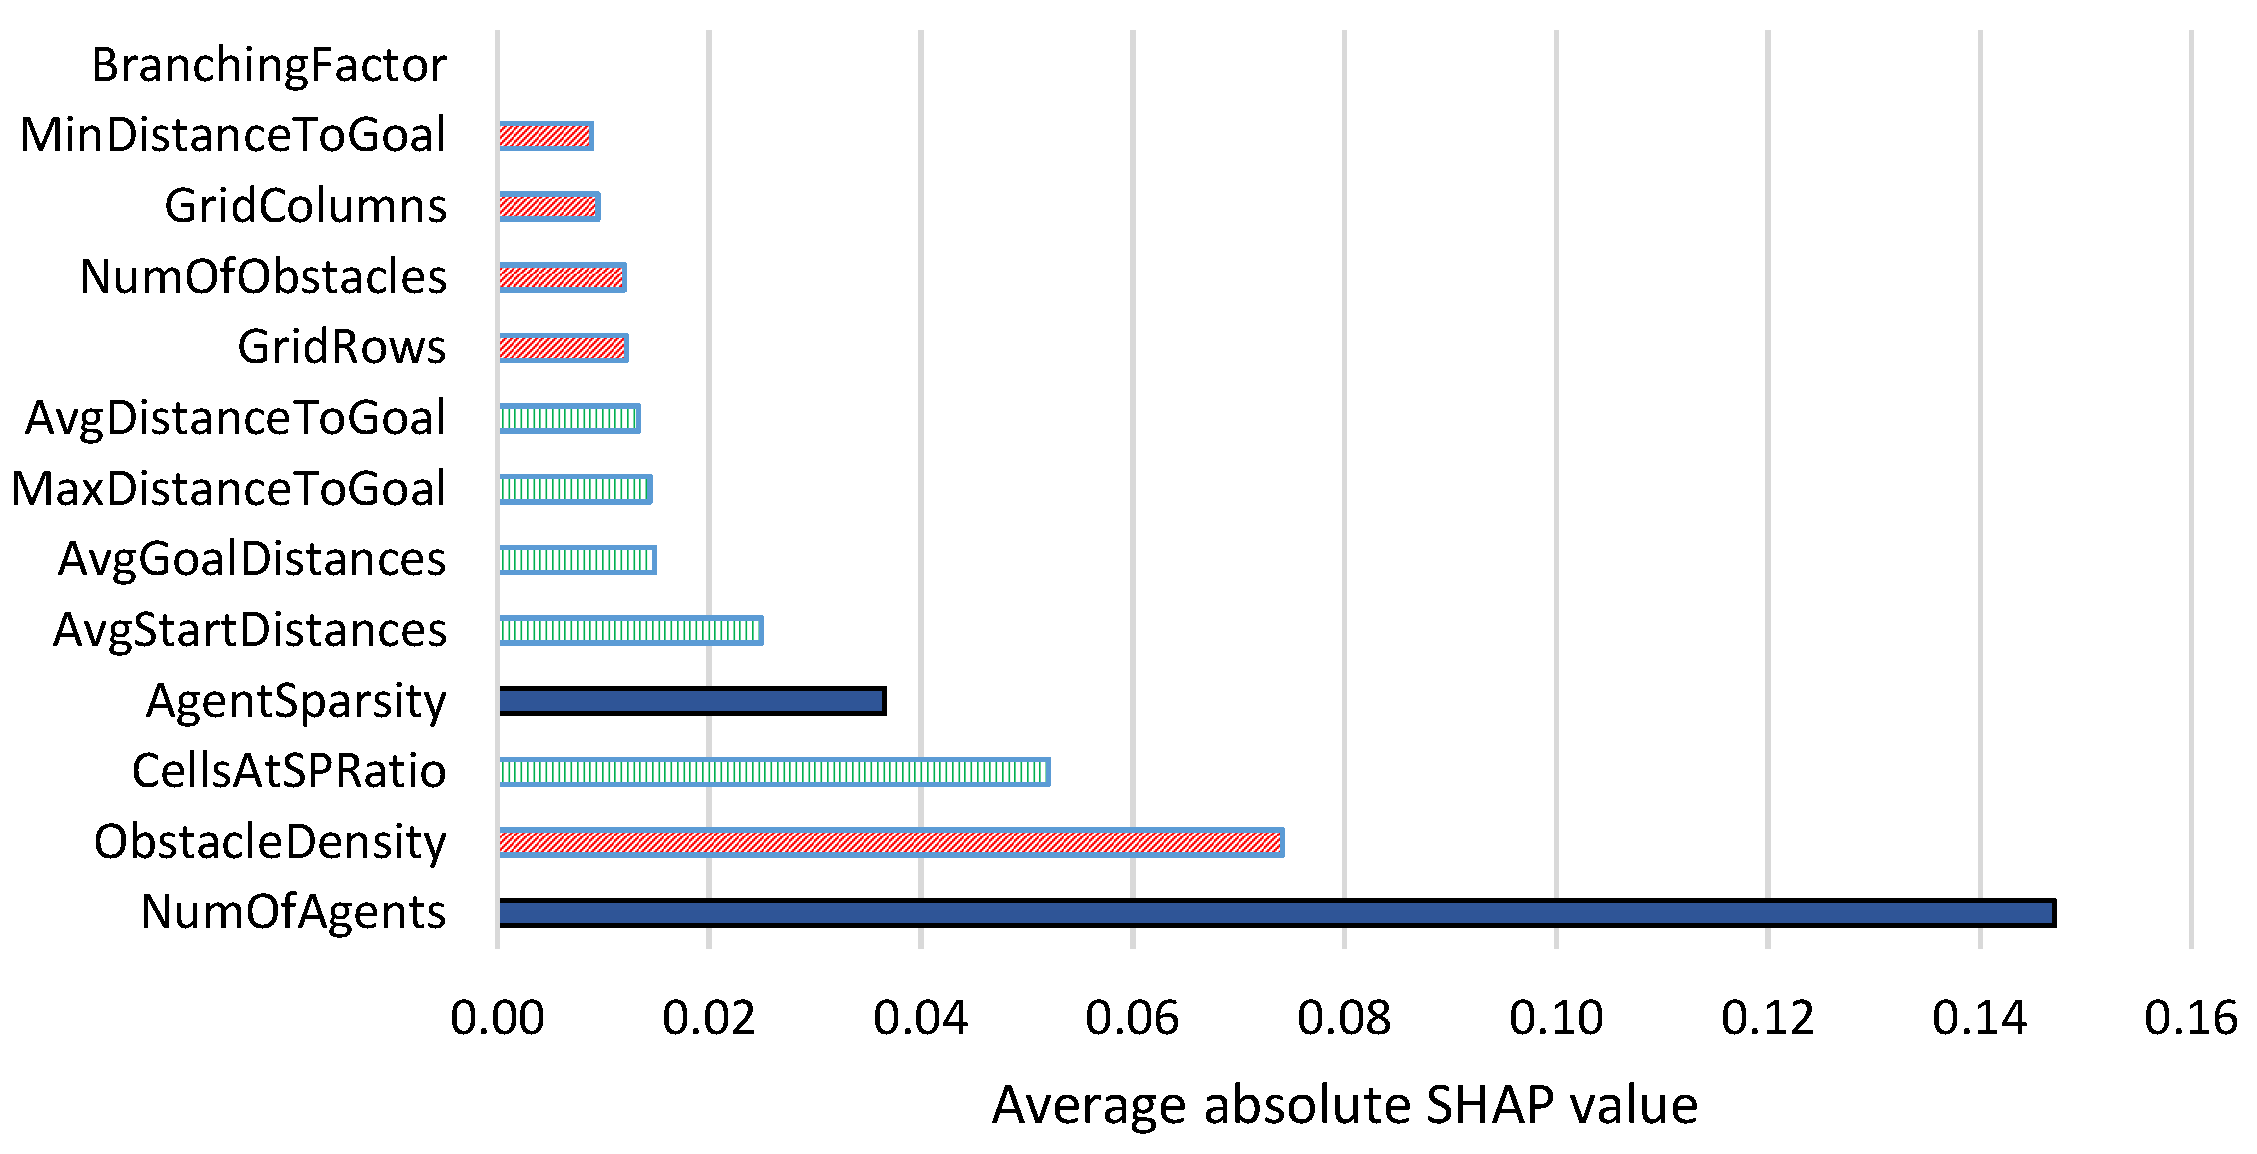
\includegraphics[width=\columnwidth]{shap-values-cropped.pdf}
    \caption{Feature importance calculated using SHAP values.} 
    %Features are sorted by their importance at y-axis. X-axis is the mean impact on model output, i.e. mean probability impact.}
    \label{fig:FeatureImportance}
\end{figure}

%To gain a higher-level understanding of the impact each feature made on the model, we computed the mean of the absolute SHAP values over all samples, features, and labels. The results are shown in Figure~\ref{fig:FeatureImportance}. As can be seen, the three most important features -- NumOfAgents, ObstacleDensity, and PointsAtSPRatio -- include a feature from each of the three feature families described in Section~\ref{sec:xgbsoot}. The key feature, as expected, is the number of agents. Of less importance are features that describe the grid itself, e.g., GridRows, NumOfObstacles, and GridColumns. Since BranchingFactor directly correlates with NumOfAgents, its importance is negligible. 
Figure~\ref{fig:FeatureImportance} shows for every feature the mean of the absolute SHAP values over all samples and labels. 
As can be seen, the three most important features -- NumOfAgents, ObstacleDensity, and PointsAtSPRatio -- include a feature from each of the three feature families described in Section~\ref{sec:xgbsoot}. The key feature, as expected, is the number of agents. Of less importance are features that describe the grid itself, e.g., GridRows, NumOfObstacles, and GridColumns. Since BranchingFactor directly correlates with NumOfAgents, its importance is negligible. 



\section{Discussion and Conclusion}
To the best of our knowledge, this is the first research on Algorithm Selection for optimal MAPF. Two high-level approaches for Algorithm Selection -- regression and classification -- as well as two types of learning algorithms -- XGBoost with handcrafted features and CNN with image-based features -- were explored. 
We implemented and evaluated these Algorithm Selection approaches on a portfolio of 6 state-of-the-art search-based optimal MAPF algorithms and a comprehensive, publicly available MAPF benchmark that includes 28 grids, resulting in a dataset of 39,000 instances. Our analysis shows that indeed Algorithm Selection can be successfully applied to optimal MAPF, yielding an optimal MAPF solver that outperforms all the optimal MAPF algorithms in its portfolio. Future work can combine feature extraction using deep learning, with the manually extracted features. Furthermore, in order to address more general MAPF problems (i.e., not only classical MAPF), graph embedding techniques may be superior to regular CNNs. 
% FutuNegular CNre work can apply more sophisticated Algorithm Selection techniques, as well as add MAPF algorithms that are not search-based to the portfolio. 



\bibliographystyle{aaai}
\bibliography{ref}

\end{document}